\section*{\huge Results}
Most of the pipeline is complete, however several things still need to be finished:
\begin{enumerate}
    \item Resolve errors in picking candidate genes for the species tree
    \item Resolve issues related to scaling up processes for large bacthes of input files
    \item Incorporate the results of markophylo into the analysis
    \item Decide on a sampling methodology for gene trees for building the phylogenetic networks
\end{enumerate}
Two networks were produced for the genera \textit{Ehrlichia} and \textit{Dehalococcoides}, using all available gene trees and the species tree for each.
\textit{Ehrlichia} contains 15 fully sequenced genomes, none of which have both Cas proteins and CRISPR arrays according to CRISPR-one.
\begin{figure}[htb!]
    \makebox[\textwidth][c]{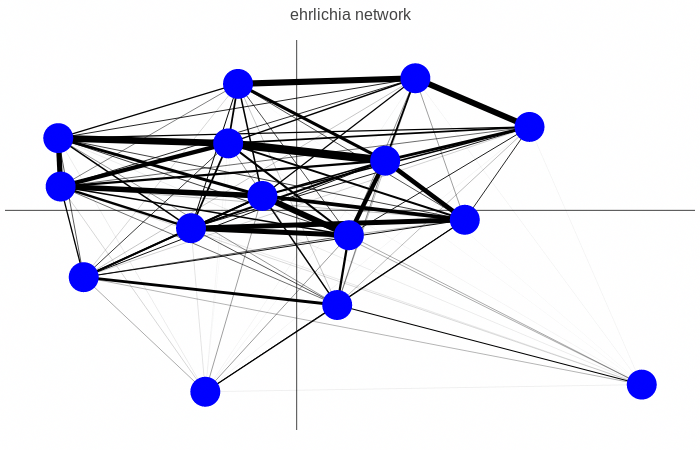
\includegraphics[width=0.8\linewidth]{ehrlichia_network.png}}
    \caption{Phylogenetic network of all strains in the genus \textit{Ehrlichia}. Blue nodes indicate no CRISPR systems. Edge thickness is proportional to the number of gene transfers estimated between strains (thicker means more transfers)}
\end{figure}
\FloatBarrier
\textit{Dehalococcoides} contains 15 fully sequenced genomes 4 of which have both Cas proteins and CRISPR arrays according to CRISPR-one.
\begin{figure}[htb!]
    \makebox[\textwidth][c]{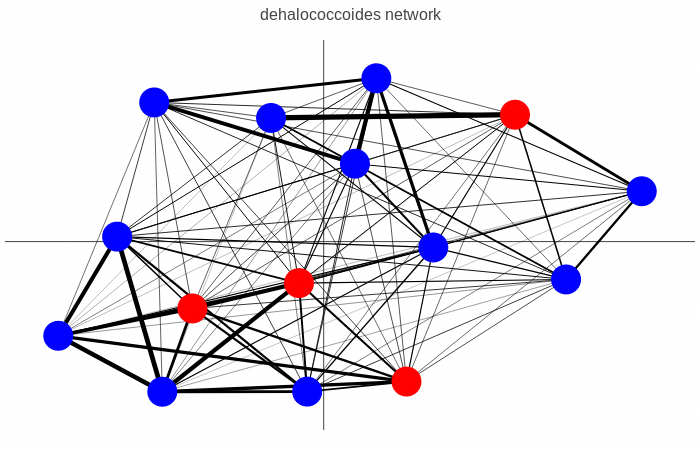
\includegraphics[width=0.8\linewidth]{dehalodeicoccus_network.png}}
    \caption{Phylogenetic network of all strains in the genus \textit{Dehalodeicoccus}. Blue nodes indicate no CRISPR systems. Edge thickness is proportional to the number of gene transfers estimated between strains (thicker means more transfers)}
\end{figure}
\FloatBarrier
From looking at these diagrams there appears to be more thick (i.e. high transfer rate) edges for \textit{Ehrlichia} than \textit{Dehalococcoides}, but the rest of the edges in \textit{Ehrlichia} are fairly thin as compared to \textit{Dehalococcoides}.
These networks do appear to be different in how they are organized, but why this is is not obvious and may be more related to the differences between these genera not related to the presence of \ac{crspc} systems.
%stats table
\begin{center}
    \begin{tabular}{l|r r}
        Metric & Ehrlichia & Dehalococcoides\\
        \hline
        Density & 0.952380952381&0.961904761905\\
        Average Edge Weight & 0.0748552512271&0.0695005449268\\
        Average Node Clustering Coefficient & 0.956&0.96\\
        Average Node Closeness Centrality & 0.9555555555555556&0.9644444444444444\\
        Average Node Communicability Betweenness Centrality & 0.5851751888088753 &0.5893446744946671\\
        Average Node Connectivity & 13.0952380952 & 13.2\\
    \end{tabular}
\end{center}
